\onecolumn
\chapter{Auswertung}
\label{ch:auswertung}

\section*{Fehlerrechnung}
Für die statistische Auswertung von $n$ Messwerten $x_i$ werden folgende Größen definiert \cite{errorSkript25}:
\begin{align}
    \bar{x} &= \frac{1}{n} \sum_{i=1}^{n} x_i \vphantom{\sqrt{\sum_i^n}^2} && \text{\textcolor{gray}{Arithmetisches Mittel}} \label{eq:arithmetisches_mittel} \\
    \sigma^2 &= \frac{1}{n-1} \sum_{i=1}^{n} (x_i - \bar{x})^2 \vphantom{\sqrt{\sum_i^n}^2} && \text{\textcolor{gray}{Variation}} \label{eq:variation} \\
    \sigma &= \sqrt{\frac{1}{n-1} \sum_{i=1}^{n} (x_i - \bar{x})^2} \vphantom{\sqrt{\sum_i^n}^2} && \text{\textcolor{gray}{Standardabweichung}} \label{eq:standardabweichung} \\
    \Delta \bar{x} &= \frac{\sigma}{\sqrt{n}} = \sqrt{\frac{1}{n(n-1)} \sum_{i=1}^n(\bar x - x_i)^2} \vphantom{\sqrt{\sum_i^n}^2} && \text{\textcolor{gray}{Fehler des Mittelwerts}} \label{eq:fehler_mittelwert} \\
    \Delta f &= \sqrt{\left(\frac{\partial f}{\partial x} \Delta x\right)^2 + \left(\frac{\partial f}{\partial y} \Delta y\right)^2} \vphantom{\sqrt{\sum_i^n}^2} && \text{\textcolor{gray}{Gauß’sches Fehlerfortpflanzungsgesetz für $f(x,y)$}} \label{eq:gauss_fehlfortpflanzung} \\
    \Delta f &= \sqrt{(\Delta x)^2 + (\Delta y)^2} \vphantom{\sqrt{\sum_i^n}^2} && \text{\textcolor{gray}{Fehler für $f = x + y$}} \label{eq:fehler_summe} \\
    \Delta f &= |a| \Delta x \vphantom{\sqrt{\sum_i^n}^2} && \text{\textcolor{gray}{Fehler für $f = ax$}} \label{eq:fehler_proportional} \\
    \frac{\Delta f}{|f|} &= \sqrt{\left(\frac{\Delta x}{x}\right)^2 + \left(\frac{\Delta y}{y}\right)^2} \vphantom{\sqrt{\sum_i^n}^2} && \text{\textcolor{gray}{relativer Fehler für $f = xy$ oder $f = x/y$}} \label{eq:relativer_fehler} \\
    \sigma &= \frac{|a_{lit} - a_{gem}|}{\sqrt{\Delta a_{lit}^2 + \Delta a_{gem}^2}} \vphantom{\sqrt{\sum_i^n}^2} && \text{\textcolor{gray}{Berechnung der signifikanten Abweichung}} \label{eq:signifikante_abweichung}
\end{align}

\twocolumn

\section{Eichkurve der Hg-Lampe}
Die Tabelle 1 des \hyperref[Protokoll]{Protokolles} zeigt die gemessenen Auslenkungen der einzelnen Spektrallinien. Ausgehend von der violetten Spektrallinie wurden die Differenzen gebildet. Der Ablehsefehler wurde auf $\Delta \alpha = 0,03 ^\circ$ geschätzt. Über diese Werte wurde eine Eichkurve erstellt, aus welcher später die Wellenlängen der Helium- und der Wasserstofflampe bestimmt werden sollen. Die Eichkurve ist in \hyperref[fig:Eichkurve]{Abbildung \ref*{fig:Eichkurve}} aufgezeichnet. Die Abzisse zeigt dabei die Wellenlänge $\lambda$ der jeweiligen Spektrallinie und die Ordinate die relative Auslenkung zur violetten Spektrallinie der Wellenlänge $\lambda = 404,7$ nm.
\begin{table}[h!]
    \centering
    \label{tab:quecksilber_spektrum}
    \hspace{-1.2cm}
    \begin{tabular}{lccc}
        \hline
        \textbf{Farbe} & \(\lambda_{\text{lit}}\, [\text{nm}]\) & \(\alpha \,[^\circ]\) & \(\text{Differenz}\,[^\circ]\) \\
        \hline
        \textcolor{red}{rot} & 690,7 & \(312,00 \pm 0,03\) & \(3,75 \pm 0,05\) \\
        \textcolor{red}{rot} & 623,0 & \(311,58 \pm 0,03\) & \(3,33 \pm 0,05\) \\
    \textcolor{orange}{gelb} & 579,1 & \(311,28 \pm 0,03\) & \(3,03 \pm 0,05\) \\
    \textcolor{orange}{gelb} & 577,0 & \(311,25 \pm 0,03\) & \(3,00 \pm 0,05\) \\
    \textcolor{green}{grün} & 546,1 & \(311,00 \pm 0,03\) & \(2,75 \pm 0,05\) \\
    \textcolor{cyan}{grünblau} & 499,2 & \(310,33 \pm 0,03\) & \(2,08 \pm 0,05\) \\
    \textcolor{cyan}{grünblau} & 491,6 & \(310,25 \pm 0,03\) & \(2,00 \pm 0,05\) \\
    \textcolor{blue}{blau} & 435,8 & \(309,17 \pm 0,03\) & \(0,92 \pm 0,05\) \\
    \textcolor{violet}{violett} & 407,8 & \(308,33 \pm 0,03\) & \(0,08 \pm 0,05\) \\
    \textcolor{violet}{violett} & 404,7 & \(308,25 \pm 0,03\) & -- \\
    \hline
\end{tabular}
\caption{Messwerte der Auslenkung des Quecksilberspektrums und der berechneten Differenzwinkel}
\end{table}

\section{Bestimmung des He-Spektrums}
Über die gemessenen Auslenkungen und die Eichkurve sollten sich nun die Wellenlängen der Spektrallinien der Heliumlampe bestimmen lassen. Der \hyperref[tab:helium_spektrum]{Tabelle \ref*{tab:helium_spektrum}} sind die Auslenkungen zu finden. Die Ungenauigkeit der Wellenlänge wird über den Fehlerschlauch bestimmt. Die größere Differenz wird als Fehler angenommen. 


\begin{table}[h!]
    \centering
    \label{tab:helium_spektrum}
    \begin{tabular}{lccc}
        \hline
        \textbf{Farbe} & \(\lambda_{\text{lit}}\, [\text{nm}]\) & \(\alpha \,[^\circ]\) & \(\text{Differenz}\,[^\circ]\) \\
        \hline
    \textcolor{violet}{violett} & 404,7 & \(308,25 \pm 0,03\) & -- \\
    \midrule
    \textcolor{blue}{blau} & 447,1 & \(309,52 \pm 0,03\) & \(1,27 \pm 0,05\) \\
    \textcolor{blue}{blau} & 471,3 & \(310,00 \pm 0,03\) & \(1,75 \pm 0,05\) \\
    \textcolor{green}{grün} & 492,2 & \(310,33 \pm 0,03\) & \(2,08 \pm 0,05\) \\
    \textcolor{green}{grün} & 501,6 & \(310,45 \pm 0,03\) & \(2,20 \pm 0,05\) \\
    \textcolor{orange}{gelb} & 587,6 & \(311,33 \pm 0,03\) & \(3,08 \pm 0,05\) \\
    \textcolor{red}{rot} & 667,8 & \(311,91 \pm 0,03\) & \(3,66 \pm 0,05\) \\
    \hline
\end{tabular}
\caption{Messwerte der Auslenkung des Heliumspektrometers und der berechneten Differenzwinkel. Violett ist der Referenzwert aus dem Quecksilberspektrum.}
\end{table}

Die aus der \hyperref[tab:helium_spektrum]{Tabelle \ref*{tab:helium_spektrum}} bestimmten Wellenlängen, die Ungenauigkeiten und die \hyperref[eq:signifikante_abweichung]{signifikanten Abweichungen (\ref*{eq:signifikante_abweichung})} sind \hyperref[tab:helium_wellenlaengen]{tabellarisch \ref*{tab:helium_wellenlaengen}} aufgelistet.
Die Auslenkungen sind in \hyperref[fig:werte]{Abbildung \ref*{fig:werte}} grün eingezeichnet.

\begin{table}[h!]
    \centering
    \label{tab:helium_wellenlaengen}
    \begin{tabular}{lccc}
        \hline
        \textbf{Farbe} & \(\lambda_{\text{lit}}\,[\text{nm}]\) & \(\lambda_{\text{gem}}\,[\text{nm}]\) & \(\sigma\text{-Abweichung}\) \\
        \hline
        \textcolor{blue}{blau} & 447,1 & \(449 \pm 4\) & 0,49 \\
        \textcolor{blue}{blau} & 471,3 & \(477 \pm 4\) & 1,69 \\
        \textcolor{green}{grün} & 492,2 & \(499 \pm 4\) & 1,74 \\
        \textcolor{green}{grün} & 501,6 & \(508 \pm 4\) & 1,59 \\
        \textcolor{orange}{gelb} & 587,6 & \(582 \pm 8\) & 0,72 \\
        \textcolor{red}{rot} & 667,8 & \(667 \pm 14\) & 0,05 \\
        \hline
    \end{tabular}
    \caption{Vergleich der gemessenen und literaturbekannten Wellenlängen des Heliumspektrums}
\end{table}




\onecolumn
\begin{figure}
    \centering
    \includegraphics[width=\textwidth, page=3]{Protokolle/33/Chapter/Messprotokoll.pdf}
    \label{fig:Eichkurve}
    \caption{Relative Auslenkung gegen die Wellenlänge der Quecksilber lampe. BEstimmung der Eichkurve (blau) und des Fehlerschlauches (orange).}
\end{figure}

\begin{figure}
    \centering
    \includegraphics[width=\textwidth, page=4]{Protokolle/33/Chapter/Messprotokoll.pdf}
    \label{fig:werte}
    \caption{Bestimmung der Wellenlängen des Helium-Spektrums (grün) und des Wasserstoff-Spektrums (lila).}
\end{figure}
\twocolumn

\section{Bestimmung des H-Spektrums und die Rydberg-Konstante}
Analog zum Helium wird das Spektrum der Wasserstofflampe bestimmt. Die Auslenkungswerte sind \hyperref[tab:auslenkung_wasserstoff]{tabellarisch \ref*{tab:auslenkung_wasserstoff}} gelistet. Diese Werte sind in \hyperref[fig:werte]{Abbildung \ref*{fig:werte}} lila eingezeichnet. 

\begin{table}
    \centering
    \label{tab:auslenkung_wasserstoff}
    \hspace{-1.1cm}
    \begin{tabular}{lccc}
        \hline
        \textbf{Farbe} & \(\lambda_{\text{lit}}\, [\text{nm}]\) & \(\alpha \,[^\circ]\) & \(\text{Differenz}\,[^\circ]\) \\
        \hline
        \textcolor{violet}{violett} & 404,7 & \(308,25 \pm 0,03\) & -- \\
        \midrule
        \textcolor{violet}{violett} & 410 & \(308,50 \pm 0,03\) & \(0,30 \pm 0,05\) \\
        \textcolor{violet}{violett} &  434 & \(309,13 \pm 0,03\) & \(0,90 \pm 0,05\) \\
        \textcolor{cyan}{türkis} & 486,1 & \(310,20 \pm 0,03\) & \(1,90 \pm 0,05\) \\
        \textcolor{red}{rot} & 656,3 & \(311,85 \pm 0,03\) & \(3,60 \pm 0,05\) \\
        \hline
    \end{tabular}
\end{table}


Die aus \hyperref[tab:auslenkung_wasserstoff]{Tabelle \ref*{tab:auslenkung_wasserstoff}} bestimmten Wellenlängen werden wieder tabellarisch festgehalten und die \hyperref[eq:signifikante_abweichung]{signifikante Abweichung (\ref*{eq:signifikante_abweichung})} zu den Literaturwerten gebildet. Die Ergebnisse sind in \hyperref[tab:e_h]{Tabelle \ref*{tab:e_h}}

\begin{table}[h!]
    \centering
    \label{tab:e_h}
    \hspace{-1.1cm}
    \begin{tabular}{lccc}
        \hline
        \textbf{Farbe} & \(\lambda_{\text{lit}}\,[\text{nm}]\) & \(\lambda_{\text{gem}}\,[\text{nm}]\) & \(\sigma\text{-Abweichung}\) \\
        \hline
        \textcolor{violet}{violett} & 410 & \(399,7 \pm 2,0\) & 0,18 \\
        \textcolor{violet}{violett} & 434 & \(429 \pm 3\) & 0,71 \\
        \textcolor{cyan}{türkis} & 486,1 & \(487,8 \pm 2,4\) & 1,50 \\
        \textcolor{red}{rot} & 656,3 & \(654,0 \pm 12,8\) & 5,20 \\
        \hline
    \end{tabular}
    \caption{Vergleich der gemessenen und literaturbekannten Wellenlängen des Heliumspektrums}
\end{table}

Über die bestimmten Wellenlängen des Wasserstofflampenspektrums lässt sich weitergehend die Rydberg-Konstante bestimmen. Dazu wird die \hyperref[eq:konst]{Gleichung \ref*{eq:konst}} umgestellt:
\begin{equation}
    R_\infty = \frac{1}{\lambda \left(\frac{1}{4} - \frac{1}{m^2}\right)}.
\end{equation}

Über die \hyperref[eq:gauss_fehlfortpflanzung]{Gauß'sche Fehlerfortpflanzung (\ref*{eq:gauss_fehlfortpflanzung})} wird sich der Fehler zu
\begin{equation}
    \Delta R_\infty = \frac{\Delta lambda}{\lambda^2 \left(\frac{}{4} - \frac{1}{m^2}\right)}
\end{equation}

berechnen, da nur $\lambda$ fehlerbehaftet ist. $m$ beschreibt die sogenannte >>Quantenzahl<<, welche sich aus dem Skript holen lässt \cite{skript25}. Die Ergebnisse für alle vier Wellenlängen der Wasserstofflampe sind in \hyperref[tab:r_werte]{Tabelle \ref*{tab:r_werte}} festgehalten.
\begin{table}
    \centering
    \begin{tabular}{c c  c c}
        \hline
        \textbf{Farbe} & \(\lambda_{\text{gem}}\,[\text{nm}]\) & $m$ & $R_\infty [\mathrm{\frac{1}{m} \cdot 10^7}]$ \\
        \hline
        \textcolor{violet}{violett} & \(399,7 \pm 2,0\) & 6 & $1,1010 \pm 0,0215$\\
        \textcolor{violet}{violett} &\(429 \pm 3\) & 5 & $1,093 \pm 0,005$ \\
        \textcolor{cyan}{türkis} & \(487,8 \pm 2,4\) & 4 & $1,110 \pm 0,009$ \\
        \textcolor{red}{rot} & \(654,0 \pm 12,8\) & 3 & $1,126 \pm 0,006$ \\
        \hline
    \end{tabular}
    \label{tab:r_werte}
\end{table}

Aus diesen wird der Mittelwert $\overline{R_\infty}$ gebildet. Sein Fehler setzt sich aus dem \hyperref[eq:fehler_mittelwert]{Fehler des Mittelwerts (\ref*{eq:fehler_mittelwert})} $\Delta \bar R_\infty$ und der quadratischen Summe der Einzelwerte zusammen:
\begin{equation}
    \Delta \overline{R_\infty} = \frac{1}{2} \sqrt{\left(\sum_{i=1}^{4} \Delta R_i^2\right) + \left(\Delta \bar R_\infty\right)^2}
\end{equation}

Somit ergibt sich final ein Wert von
\begin{equation}
\boxed{
    \overline{R_\infty} = (1,11 \pm 0,17) \, \mathrm{\frac{1}{m} \cdot 10^7}
}
\end{equation}

Die Abweichung zum Literaturwert beträgt somit:
\begin{equation}
    \frac{\left| \overline{R_\infty} - R_{lit} \right|}{\Delta \overline{R_\infty}} = 0,06 \sigma
\end{equation}  